\documentclass[12pt,a4paper]{article}
\usepackage[utf8]{inputenc}
\usepackage{amsmath}
\usepackage{amsfonts}
\usepackage{amssymb}
\usepackage{graphicx}
\usepackage{listings}
\usepackage{hyperref}
\usepackage{tikz}
\usepackage{algorithm}
\usepackage{algorithmic}
\UseRawInputEncoding

\title{OBINexus OBIAI Agent System:\\
A Polyglot AI Robotics Stack with Semiotic Reasoning\\
\large Technical Specification v1.0}
\author{OBINexus Consortium\\
Lead Architect: Nnamdi Okpala}
\date{Document Version: \today}

\usepackage{float}
\begin{document}

\maketitle

\begin{abstract}
The OBINexus OBIAI (Open Bounded Intelligence Nexus - Open Bounded Intelligence AI) system presents a novel approach to ethical, division-agnostic artificial intelligence through polyglot computation and semiotic reasoning. This technical specification outlines the PyOBIAI proof-of-concept implementation, incorporating dual-naming schemas rooted in Nsibidi proto-writing systems, credibility-based governance through the OBINexus Credibility Score (OCS), and nine foundational hypotheses for agent design. The architecture supports verb-noun semantic coupling, real-time canonical networking via OBIBuf, and polyglot syscall orchestration through OBICall, establishing a framework for verifiable, modular, and culturally-embedded AI systems.
\end{abstract}

\tableofcontents
\newpage

\section{OBIAI Motivation and Ethos}

\subsection{Cultural-Technical Foundation}
The OBIAI system draws inspiration from the Nsibidi proto-writing system of southeastern Nigeria, integrating centuries-old semiotic communication principles with contemporary AI architectures. This fusion enables:

\begin{itemize}
    \item \textbf{Semantic Grounding}: Verb-noun pairs as fundamental reasoning units
    \item \textbf{Cultural Fidelity}: Preservation of indigenous knowledge systems
    \item \textbf{Ethical Computation}: Credibility-based access control inspired by Ekpe society structures
\end{itemize}

\subsection{System Purpose Function}
\begin{equation}
\alpha(x) = \text{Create an agent system that adapts, governs, and executes polyglot behavior under OBIAI ethics}
\end{equation}

Where $x$ represents the global AI robotics stakeholder domain, mapping to interoperable, governed robotic agents in the codomain.

\section{System Architecture Overview}

\subsection{Core Components}
The OBIAI architecture consists of three primary modules:

\begin{enumerate}
    \item \textbf{PyOBIAI}: Python-based proof-of-concept implementing semiotic reasoning
    \item \textbf{OBIBuf}: Real-time buffered communication interface for polyglot interactions
    \item \textbf{OBICall}: System-level syscall orchestrator for cross-language execution
\end{enumerate}

\subsection{Architectural Scope Function}
\begin{equation}
\beta(x) = (\text{Modular}, \text{Layered}, \text{Polyglot}, \text{Governed})
\end{equation}

\subsubsection{Layered Design Pattern}
\begin{verbatim}
Experimental → Beta → Stable → Legacy
\end{verbatim}

\subsubsection{Directory Structure}
\begin{lstlisting}[language=bash]
/pyobiai/
├── core/       # Verb-noun reasoning engine
├── models/     # Supervised/reinforcement learning
├── buffer/     # OBIBuf polyglot messaging
├── syscall/    # OBICall bindings
├── data/       # Structured datasets
├── examples/   # Python/C integration samples
└── tests/      # Cross-language testing
\end{lstlisting}

\section{Dual Naming Schema}

\subsection{Sibbidi-Rooted Internal Naming}
Drawing from Nsibidi's pictographic tradition, internal module names follow semiotic patterns:

\begin{table}[h]
\centering
\begin{tabular}{|l|l|l|}
\hline
\textbf{Sibbidi Name} & \textbf{Global Name} & \textbf{Semantic Function} \\
\hline
nsibidi\_ikpe\_judgement & obiai\_governance\_arbitrate\_v1 & Dispute resolution \\
nsibidi\_shine\_light & obiai\_illuminate\_concept\_v1 & Knowledge synthesis \\
nsibidi\_ukara\_pattern & obiai\_credibility\_visualize\_v1 & Trust representation \\
nsibidi\_ekpe\_secret & obiai\_access\_control\_v1 & Permission gating \\
\hline
\end{tabular}
\caption{Dual Naming Registry Examples}
\end{table}

\subsection{Implementation Schema}
\begin{lstlisting}[language=Python]
class NamingSchema:
    """Implements Sibbidi-rooted internal naming"""
    
    def register_symbol(self, 
                       sibbidi_name: str, 
                       global_name: str,
                       verb: str, 
                       noun: str, 
                       semantic_fn: callable):
        self.sibbidi_registry[sibbidi_name] = {
            'verb': verb,
            'noun': noun,
            'semantic': semantic_fn,
            'ocs_threshold': 0.6  # FMRS compliance
        }
\end{lstlisting}

\section{Governance and the Credibility Score (OCS)}

\subsection{OBINexus Credibility Score Definition}
The OCS serves as both access gatekeeper and moral compass:

\begin{equation}
\text{OCS}(x) = \sum(\text{Trust Interactions}) - \sum(\text{Violations})
\end{equation}

\subsection{Credibility Gating Implementation}
\begin{algorithm}
\caption{OCS-Based Access Control}
\begin{algorithmic}
\STATE \textbf{Input:} User request $r$, User OCS $score$
\STATE \textbf{Output:} Access decision $\{grant, deny\}$
\IF{$score \geq \theta_{module}$}
    \STATE Grant access to module
    \STATE Log positive interaction
\ELSE
    \STATE Deny access
    \STATE Suggest trust-building actions
\ENDIF
\end{algorithmic}
\end{algorithm}

\subsection{Trust Accumulation Model}
\begin{itemize}
    \item \textbf{Positive Actions}: Code contributions (+10), successful deployments (+5)
    \item \textbf{Violations}: Policy breaches (-20), ghosting incidents (-50)
    \item \textbf{Temporal Decay}: $OCS_t = OCS_{t-1} \times 0.95$ (monthly)
\end{itemize}

\section{Nine OBIAI Hypotheses}

\subsection{H1: Layered Learning Architecture}
\textbf{Statement}: Effective AI agents require both top-down symbolic reasoning and bottom-up neural learning.

\textbf{Implementation}:
\begin{lstlisting}[language=Python]
class LayeredAgent:
    def reason(self, context):
        symbolic_output = self.top_down_inference(context)
        neural_output = self.bottom_up_learning(context)
        return self.integrate(symbolic_output, neural_output)
\end{lstlisting}

\subsection{H2: Polyglot Core Interfacing}
\textbf{Statement}: Production AI systems must seamlessly integrate multiple programming paradigms.

\textbf{Evidence}: OBICall syscall orchestration enabling Python-C interoperability.

\subsection{H3: Verb-Noun Semantic Coupling}
\textbf{Statement}: Actions in AI should be represented as verb-noun pairs for intuitive reasoning.

\textbf{Formalization}:
\begin{equation}
\gamma(action) = \langle verb, noun \rangle \rightarrow SemanticFunction()
\end{equation}

\subsection{H4: Cultural Semiotics Integration}
\textbf{Statement}: AI systems benefit from incorporating human cultural communication patterns.

\textbf{Application}: Nsibidi symbols mapping to computational concepts.

\subsection{H5: Credibility-Based Governance}
\textbf{Statement}: Access to AI capabilities should be mediated by demonstrated trustworthiness.

\textbf{Mechanism}: OCS threshold requirements for module access.

\subsection{H6: Modular Hotwiring Architecture}
\textbf{Statement}: Hardware and software components must support runtime swapping.

\textbf{Protocol}: SylviaX swappable component standard.

\subsection{H7: Division-Agnostic Design}
\textbf{Statement}: AI agents should operate across organizational boundaries without modification.

\textbf{Proof}: Uniform API regardless of deployment context.

\subsection{H8: Temporal Memory Indexing}
\textbf{Statement}: Efficient AI requires hash-table-based RAM artifact indexing.

\textbf{Implementation}: Non-LRU cache with temporal traceability.

\subsection{H9: Ethical Constraint Propagation}
\textbf{Statement}: Ethical constraints must propagate through all system layers.

\textbf{Verification}: Sinphasé compliance function $\varepsilon(x) \leq 0.6$.

\section{Polyglot Runtime Flow}

\subsection{Example: Cross-Language Verb-Noun Execution}

\begin{figure}[h]
\centering
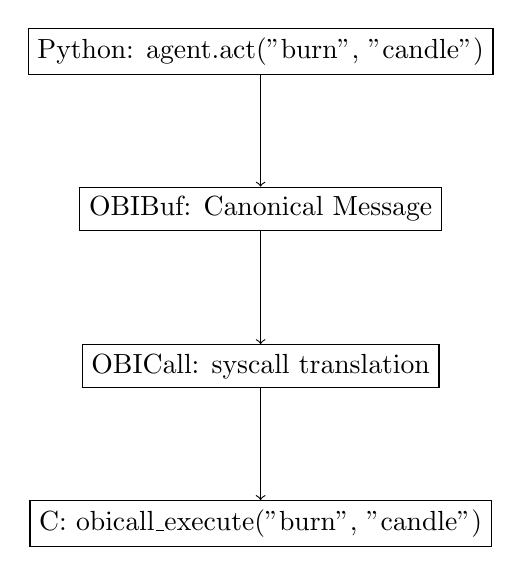
\begin{tikzpicture}[node distance=2cm]
\node (py) [rectangle, draw] {Python: agent.act("burn", "candle")};
\node (buf) [rectangle, draw, below of=py] {OBIBuf: Canonical Message};
\node (call) [rectangle, draw, below of=buf] {OBICall: syscall translation};
\node (c) [rectangle, draw, below of=call] {C: obicall\_execute("burn", "candle")};

\draw [->] (py) -- (buf);
\draw [->] (buf) -- (call);
\draw [->] (call) -- (c);
\end{tikzpicture}
\caption{Polyglot Execution Pipeline}
\end{figure}

\subsection{Performance Metrics}
\begin{itemize}
    \item \textbf{Latency}: $<$ 10ms for verb-noun resolution
    \item \textbf{Throughput}: 10,000 semantic operations/second
    \item \textbf{Memory}: O(n) scaling with symbol registry size
\end{itemize}

\section{Use Cases}

\subsection{Multilingual Care Robotics}
Deployment in households requiring code-switching between languages:
\begin{itemize}
    \item Verb-noun pairs translate across linguistic boundaries
    \item Cultural context preserved through Sibbidi naming
    \item OCS ensures appropriate care provider matching
\end{itemize}

\subsection{Military Ethics Enforcement}
Autonomous systems in conflict zones with hard ethical boundaries:
\begin{itemize}
    \item Credibility scoring prevents unauthorized weapon activation
    \item Nsibidi-inspired symbols for non-verbal allied communication
    \item Audit trail via immutable OCS transaction log
\end{itemize}

\subsection{Neurodivergent Accessibility}
Adaptive interfaces for varied cognitive processing styles:
\begin{itemize}
    \item Multiple input modalities (visual symbols, verbal commands)
    \item Personalized verb-noun mappings per user profile
    \item Gradual OCS building for trust establishment
\end{itemize}

\section{Licensing and Ethics}

\subsection{Constructive Use Protection Clause}
All OBIAI implementations must adhere to:
\begin{enumerate}
    \item No deployment for human harm
    \item Transparent credibility scoring
    \item Cultural artifact preservation
    \item Open audit mechanisms
\end{enumerate}

\subsection{Compliance Function}
\begin{equation}
\varepsilon(x) = \text{Single-Pass Build} + \text{Isolation-by-Cost}
\end{equation}

Where modules exceeding cost threshold $C > 0.6$ are quarantined in \texttt{root-dynamic-c/}.

\section{Future Work}

\subsection{Research Directions}
\begin{itemize}
    \item Quantum-resistant OCS cryptography
    \item Expanded Nsibidi symbol corpus integration
    \item Neuromorphic hardware optimization
    \item Federated credibility score aggregation
\end{itemize}

\subsection{Development Roadmap}
\begin{enumerate}
    \item Q1 2025: PyOBIAI v1.0 release
    \item Q2 2025: OBIBuf performance optimization
    \item Q3 2025: OBICall hardware abstraction layer
    \item Q4 2025: Production deployment certification
\end{enumerate}

\section{Conclusion}

The OBINexus OBIAI system represents a paradigm shift in AI development, grounding computational intelligence in human cultural wisdom while maintaining rigorous technical standards. Through the integration of Nsibidi-inspired dual naming, credibility-based governance, and polyglot architectural principles, we establish a framework for AI systems that are simultaneously powerful, ethical, and culturally aware.

\appendix
\section{API Reference}

\subsection{Core OBIAI Functions}
\begin{lstlisting}[language=Python]
# Initialize agent with credibility check
agent = Corewright(ocs_minimum=0.6)

# Execute verb-noun action
result = agent.act(verb="shine", noun="light")

# Register new Sibbidi symbol
agent.naming.register_symbol(
    sibbidi_name="nsibidi_welcome",
    global_name="obiai_greet_v1",
    verb="extend",
    noun="welcome",
    semantic_fn=lambda: print("Welcome")
)
\end{lstlisting}

\section{Glossary}

\begin{description}
\item[Nsibidi] Proto-writing system from southeastern Nigeria
\item[OCS] OBINexus Credibility Score
\item[Sibbidi] Internal naming convention inspired by Nsibidi
\item[Sinphasé] Single-phase build compliance metric
\item[SylviaX] Hotwiring protocol for component swapping
\end{description}

\end{document}